\documentclass{standalone}
\usepackage{graphicx, standalone}
\usepackage[compat=1.1.0]{tikz-feynman}
\usepackage{tikz}
\usepackage{amsmath, amssymb, bm}
\usepackage{euler}
\usepackage{fontspec}
\setmainfont{MinionPro}
\usepackage{comment}

\newcommand{\mmin}{\ensuremath M_{\text{min}}}
\newcommand{\mmax}{\ensuremath M_{\text{max}}}
\newcommand{\nmin}{\ensuremath N_{\text{min}}}
\newcommand{\nmax}{\ensuremath N_{\text{max}}}
\newcommand{\q}{\ensuremath\text{q}}
\renewcommand{\l}{\ensuremath\text{L}}
\newcommand{\h}{\ensuremath\text{H}}

\begin{document}

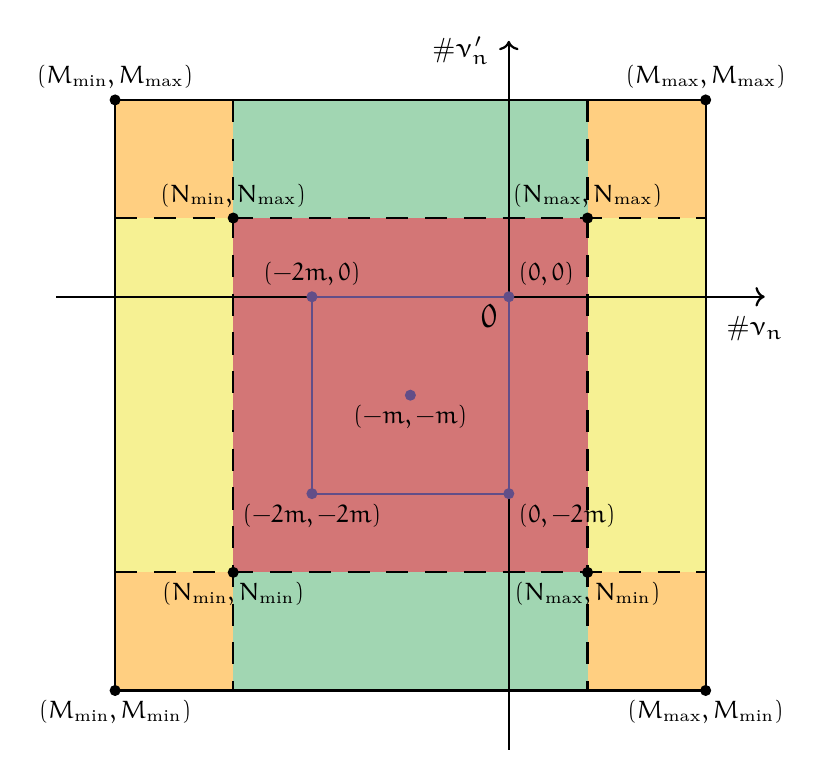
\begin{tikzpicture}[baseline=(current bounding box.center)]
    % Define colors
    \definecolor{customred}{RGB}{211, 118, 118}
    \definecolor{customgreen}{RGB}{161, 214, 178}
    \definecolor{customblue}{RGB}{98, 78, 136}
    \definecolor{customyellow}{RGB}{246, 241, 147}
    \definecolor{customorange}{RGB}{255, 207, 129}
    
    \def\innerwidth{2.25}
    \def\outerwidth{1.5}
    \def\fullwidth{3.75}
    \def\mwidth{1.25}
    
    \coordinate (a1) at (-\fullwidth,\fullwidth);
    \coordinate (a2) at (-\fullwidth,\innerwidth);
    \coordinate (a3) at (-\fullwidth,-\innerwidth);
    \coordinate (a4) at (-\fullwidth,-\fullwidth);
    
    \coordinate (b1) at (-\innerwidth,\fullwidth);
    \coordinate (b2) at (-\innerwidth,\innerwidth);
    \coordinate (b3) at (-\innerwidth,-\innerwidth);
    \coordinate (b4) at (-\innerwidth,-\fullwidth);
    
    \coordinate (c1) at (\innerwidth,\fullwidth);
    \coordinate (c2) at (\innerwidth,\innerwidth);
    \coordinate (c3) at (\innerwidth,-\innerwidth);
    \coordinate (c4) at (\innerwidth,-\fullwidth);
    
    \coordinate (d1) at (\fullwidth,\fullwidth);
    \coordinate (d2) at (\fullwidth,\innerwidth);
    \coordinate (d3) at (\fullwidth,-\innerwidth);
    \coordinate (d4) at (\fullwidth,-\fullwidth);
    
    \coordinate (m1) at (-\mwidth,\mwidth);
    \coordinate (m2) at (\mwidth,\mwidth);
    \coordinate (m3) at (\mwidth,-\mwidth);
    \coordinate (m4) at (-\mwidth,-\mwidth);
    \coordinate (m0) at (0,0);

    % Color the quadrants
    \fill[customred] (b2) rectangle (c3);
    \fill[customgreen] (b1) rectangle (c2);
    \fill[customgreen] (b3) rectangle (c4);
    \fill[customyellow] (a2) rectangle (b3);
    \fill[customyellow] (c2) rectangle (d3);
    \fill[customorange] (a1) rectangle (b2);
    \fill[customorange] (c1) rectangle (d2);
    \fill[customorange] (a3) rectangle (b4);
    \fill[customorange] (c3) rectangle (d4);
    
    % Draw axis lines
    \draw[thick, ->] (-4.5,\mwidth) -- (4.5,\mwidth);
    \draw[thick, ->] (\mwidth,-4.5) -- (\mwidth,4.5);
    
    % Draw the outer boundary
    \draw[thick, black] (a1) -- (d1) -- (d4) -- (a4) -- (a1);
    
    % Draw the inner boundary
    %\draw[thick, dashed] (b2) -- (c2) -- (c3) -- (b3) -- (b2);
    
    % Draw the inner m region
    \draw[thick, customblue] (m1) -- (m2) -- (m3) -- (m4) -- (m1);
    
    % Draw the outer boundaries
    \draw[thick, dash pattern=on 8pt off 6pt] (b1) -- (b4);
    \draw[thick, dash pattern=on 8pt off 6pt] (c1) -- (c4);
    \draw[thick, dash pattern=on 8pt off 6pt] (a2) -- (d2);
    \draw[thick, dash pattern=on 8pt off 6pt] (a3) -- (d3);
    
    % Draw grid dots
    \foreach \x in {-\fullwidth,\fullwidth} { \foreach \y in {-\fullwidth,\fullwidth} {
        \fill[black] (\x,\y) circle (2pt);
    }}
    
    \foreach \x in {-\innerwidth,\innerwidth} { \foreach \y in {-\innerwidth,\innerwidth} {
        \fill[black] (\x,\y) circle (2pt);
    }}

    \foreach \x in {-\mwidth,\mwidth} { \foreach \y in {-\mwidth,\mwidth} {
        \fill[customblue] (\x,\y) circle (2pt);
    }}
    \fill[customblue] (0,0) circle (2pt);
    
    % Labels
    \node at (\mwidth-0.25,\mwidth-0.25) {\large $0$};
    \node[left] at (1.125,4.375) {$\#\nu'_n$};
    \node[below] at (4.375,1.125) {$\#\nu_n$};
    
    \node[above] at (d1) {\small $(\mmax, \mmax)$};
    \node[above] at (a1) {\small $(\mmin, \mmax)$};
    \node[below] at (a4) {\small $(\mmin, \mmin)$};
    \node[below] at (d4) {\small $(\mmax, \mmin)$};
    
    \node[above] at (c2) {\small $(\nmax, \nmax)$};
    \node[above] at (b2) {\small $(\nmin, \nmax)$};
    \node[below] at (b3) {\small $(\nmin, \nmin)$};
    \node[below] at (c3) {\small $(\nmax, \nmin)$};
    
    \node[above right] at (m2) {\small $(0,0)$};
    \node[above] at (m1) {\small $(-2m,0)$};
    \node[below] at (m4) {\small $(-2m,-2m)$};
    \node[below right] at (m3) {\small $(0,-2m)$};
    \node[below] at (m0) {\small $(-m,-m)$};
\end{tikzpicture}
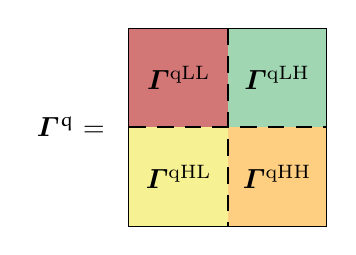
\begin{tikzpicture}[baseline=(current bounding box.center)]
	\definecolor{customred}{RGB}{211, 118, 118}
    \definecolor{customgreen}{RGB}{161, 214, 178}
    \definecolor{customyellow}{RGB}{246, 241, 147}
    \definecolor{customorange}{RGB}{255, 207, 129}
    
    \def\width{1.25};
    
    \coordinate (a1) at (-\width,\width);
    \coordinate (a2) at (-\width,0);
    \coordinate (a3) at (-\width,-\width);
    
    \coordinate (b1) at (0,\width);
    \coordinate (b2) at (0,0);
    \coordinate (b3) at (0,-\width);
    
    \coordinate (c1) at (\width,\width);
    \coordinate (c2) at (\width,0);
    \coordinate (c3) at (\width,-\width);
    
    
	\node [left=0.2 of a2] {$\bm\Gamma^{q}=$};
	
	% Draw the matrix square
    \draw[thick] (a1) rectangle (c3);
    
    % Color the quadrants
    \fill[customred] (a1) rectangle (b2);
    \fill[customgreen] (c1) rectangle (b2);
    \fill[customyellow] (a3) rectangle (b2);
    \fill[customorange] (c3) rectangle (b2);
    
    % Matrix entries
    \node at ($(a1)!0.5!(b2)$) {$\bm\Gamma^{\q\l\l}$};
    \node at ($(c1)!0.5!(b2)$) {$\bm\Gamma^{\q\l\h}$};
    \node at ($(a3)!0.5!(b2)$) {$\bm\Gamma^{\q\h\l}$};
    \node at ($(c3)!0.5!(b2)$) {$\bm\Gamma^{\q\h\h}$};
    
    \draw[thick, dash pattern=on 6pt off 4pt] (a2) -- (c2);
    \draw[thick, dash pattern=on 6pt off 4pt] (b1) -- (b3);
\end{tikzpicture}

\end{document}